\chapter{Related Work}
\label{cha:related-work}
This chapter presents different works done in areas which is related to this project. It includes both some research work and some implemented work. 
The different sections presented in this chapter will be divided into following areas:
\begin{enumerate}
	\item Existing peer-to-peer networks
	\item Existing group communication within peer-to-peer  
	%\item Confidentiality and privacy in communication
\end{enumerate}

\section{Peer-to-Peer Networks}
\label{sec:p2p-networks}
Peer-to-Peer (P2P) networking has been evolving for some decades and is now a solid alternative for the existing centralized approach of communicating.
P2P is characterized by sharing resources directly between peers without any intermediate interaction and does not have any single point of failure. The activities are coordinated between the peers in the network.
There are many existing solutions for P2P networks. In the coming subsections a few of these networks, which are relevant for this project, are presented. 

Many P2P systems are implemented as Distributed Hash Tables (DHT) which are a distributed key-value store \cite{stoica2001chord}.
DHT provides look-up services similar to regular hash tables.
DHT also provides a good load balance by distributing key-values evenly between peers which is an important factor for P2P systems.

\subsection{Pastry}
Pastry is a structured P2P network, that implements DHT, designed to be a scalable and fault-tolerant infrastructure for other applications \cite{rowstron2001pastry}. 
%The keys and the values are stored in the peers and these can then be used to build knowledge about the peers in the network.
Each peer in the network has a routing table which provides some knowledge about the other peers in the network. These routing tables are also maintained by each peer.
The routing table consists of a list of peers with unique id's mapping to the addresses of some peers in the network.
If a peer receives a lookup request it will use the routing table to find a concrete peer also known as node by routing through the nodes with closest id's.

The routing table used in Pastry is based on prefix matching and consists of three layers; \emph{Leaf set}, \emph{Routing table}, and \emph{Neighborhood set}. These layers are visualized in \autoref{fig:pastryrouting}.
\begin{figure}[bth]
\includegraphics[width=1\linewidth]{gfx/pastry-routing}
\caption[Routing table for Pastry]{Routing table for Pastry} \label{fig:pastryrouting}
\end{figure}

When a message is send to a specific node this node's id is looked up in the routing table, where it first will check if the key fits in the range of it's \emph{leaf set}. If the key is not covered by the \emph{leaf set} the \emph{routing table} inside the Pastry routing table is used to forward the message to a node that shares a common prefix. 

Pastry routes with O(log\textsubscript{2\textsuperscript b} N) routing hops. A trade-off between the maximum number of hop and the size of the \emph{routing table} is configured by a configuration parameter ``b''.
An advantage in Pastry is that it prefers nodes that are close in the ip-space and thereby gives a high performance in the real world.

%with the key by at least one digit.
%In rare cases where the appropriate entry in the routing table is empty or the matched node is unreachable, the message will again be forwarded using the routing table to a node which shares a common prefix and is numerically closer  to the key than the previous node's id.
%a message can be forwarded to the nearest destination node.

%Responsible for the keys closest to the peer..
%Structure knowledge that the individual peer has about the rest of the network
%route 
%use peer you know

\subsection{Kademlia}
Kademlia is another structured P2P network functioning as a DHT \cite{maymounkov2002kademlia}. Kademlia focuses on scalability, load-balancing, and fault-tolerance. Kademlia is used in many applications with millions of users including \emph{BitTorrent}.

Every Kademlia node owns a 160-bit long unique identifier. The keys are stored at the node with equal id or with the shortest distance.
The distance between nodes is determined using bitwise \emph{exclusive OR} (XOR). The XOR is unidirectional and it therefore ensure a unique distance for every node. Unidirectionality means that all lookups for a specific key end at the same path, regardless of the originating node, enabling caching frequently requested key-values and thus lessens the load on nodes with popular contents.

Nodes in Kademlia is treated as leaves in a binary tree. The position of nodes is determined by the shortest unique prefix of its ID as illustrated by \autoref{fig:kademliaprefix}. 

\begin{figure}[bth]
	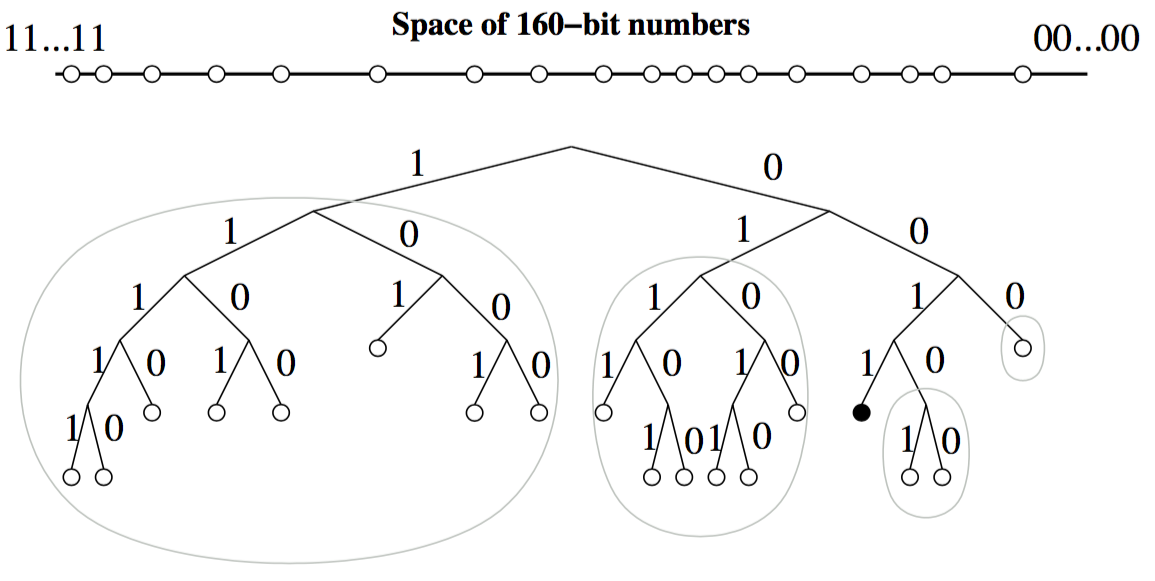
\includegraphics[width=1\linewidth]{gfx/kademlia-tree}
	\caption[Kademlia Binary tree]{Kademlia Binary tree} \label{fig:kademliaprefix}
\end{figure}

Every node see the rest of the binary tree as divided subtrees. The closest subtree consists of nodes with an id that share the longest common prefix with the node. Every node is ensured to know at least one node in each of the subtrees. That info is stored in the k-bucket, which is used for the lookup process. When a node receives a lookup request it will search for a node inside its bucket which shares the longest common prefix with the lookup-key. The discovered node is then used to another lookup request. This process is repeated iteratively until the required node is reached.

Kademlia stands out from the other DHT P2P systems by maintaining the routing tables with a minimal effort. Everytime a node receives a request it will update its k-bucket with info about the requesting node. Thus the k-bucket will stay up-to-date without any manual effort. This is a big advantage compared with Pastry which uses a huge amount of control-traffic to maintain it's routing table.

%Unlike Pastry, Kademlia uses lookups for discovering a message receiver, and thus a sender first finds the correct message receiver using lookup messages and then directly sends the message to the node. 

%While Kademlia may flood the network with lookups, it does not flood the network with control messages; however, this together may generate more data traffic.

\subsubsection{TomP2P}
TomP2P is a JAVA implementation of Kademlia protocol with many extra features \cite{TomP22:online}. TomP2P allows for instance automatic set up of NAT traversal which can solve the challenge with unreachable external peers. This is important when using TomP2P as an infrastructure for cross-platform applications that among others run on mobile devices.

TomP2P enables custom behaviour for built-in methods like \emph{GET} and \emph{PUT}. Thus developers is able to write some custom code to be executed when a key-value for instance is requested.

Replication in TomP2P is categorized as indirect replication and direct replication. The direct replication is the original replication mechanism defined in the Kademlia design where each node constantly publish its content to the closest nodes. The indirect replication is about extending the responsibility of the publishing functionality by also making the neighbours contribute.
    
The security implementation in TomP2P ensures data integrity, which means preventing unauthorized users to alter the stored key-values. This is done by using the author's public key to sign the key-values.

Encrypted communication is not a part of TomP2P and thereby confidentiality is not ensured by default.

%Each TomP2P node has a table that can be configured either to be disk-based or memory-based to store its values. 

\section{Group Communication}
Group communication is an important aspect of communication and can be used to a number of useful things as group chat, live media stream etc.
Regular DHT's or structured networks does not support group communication per default, but there has been build different extensions which supports multi-casting and thereby making it possible to establish communication between certain group of nodes in the network \cite{p2poverlay} \cite{trustedp2p} . 
A tree structure is normally used for supporting multicast functionality, where the tree ensures the relation between nodes associated to the group. This tree structure can be build in different ways depending on the trade-off's between speed, load-balancing, and ordering.

The top-down approach of building a tree is about using the root to distribute data to other group members in the tree. This means that everytime a peer needs to join, send or leave a group it need to contact the root of the group and afterwards the root will initiate the multicasting. This approach ensures by default a correct ordering of the communicated messages. 

The crawl approach of building a tree is to make the members of the tree forward the messages to their children and parents without using any central nodes. Thus all nodes in the tree are equally loaded and the messages are distributed faster in the network in contrast to the top-down approach. However the sequence of the messages is hard to maintain. 

\subsection{SCRIBE}
SCRIBE is a very well-known extension build on top of Pastry which supports group communication. 
The tree which is build by SCRIBE is not a part of Pastry, but it is build on top of Pastry. SCRIBE has implemented the top-down approach. 

To create a group in SCRIBE a \emph{groupID} is generated and a ``create'' message is then routed in the Pastry network to the node whose ID is closest to the \emph{groupID}. This receiving node becomes the root and it will keep the \emph{groupID} saved as a normal key-value pair.

To join a created group a ``join'' message is send towards the \emph{groupID}, then a node in the Pastry network will receive the message and add the sending node as a child and if this parent node is not a forwarder it will send a ``join'' message towards the \emph{groupID} and thus become a forwarder for the group. This means that a group consists both of group members and forwarders. Every node in a group is a forwarder, but a forwarder is not necessarily a member of  the group. 

To leave a group, a node will first check if it has any children and if it hasn't is sends a ``leave'' message to its parent which continuous recursively up the tree otherwise it stays as forwarder but not a member.

 
\subsection{Kademlia Group Extension}
A research article presents an extension to the Kademlia network that provides group communication \cite{matl2015effective}. This article is inspired from SCRIBE and uses many of the same elements used in SCRIBE. The article discusses two tree-architectures; the first one is the top-down approach also used in SCRIBE and the second one is the crawl approach.

The Kademlia extension uses in their case study the crawl approach for building its tree and compares it with SCRIBE. Measurements are made for message delay when multicasting messages and the amount of transferred data. The results from the case study shows that there is not much difference in the message delay between the two systems even though the crawl approach was expected to be faster than the top-down approach. The reason could be that Pastry piggy-backs the messages in the lookup request and thereby saves some time. However, the results for the other measurements are as expected where SCRIBE uses more data than the Kademlia extension because of the huge amount of data sent for maintaining the routing table in Pastry.

%case study - crawl is used
The article also discusses how to keep the tree fault-tolerant and proposes that every tree member should periodically send a control message to its parent. Another aspect is if a root member fails, which is a major problem. For maintaining the tree root, multiple roots are presented such that the duplicated root can replace the original root in case it fails.


%\section{Confidential Communication}
%Keeping the communication private from external people is depending on two factors; the first one is that the group members agrees on a secret key only known by the group members and the second factor is to encrypt the communication using the agreed secret key.
% 
%\subsection{Encrypted Communication}
%Encrypted communication is used for obtaining confidentiality such a third party cannot intercept the communication. By using encryption, data can be kept secret between a certain group of people.
%TODO: Not done yet

%%Asymetric
%\textbf{Asymmetric encryption:} Sometime it is only necessary to encrypt asymetrically.
%
%%Symetric
%\textbf{Symmetric encryption:} 

%\subsection{Key Exchange}
%\subsubsection{Diffie-Hellman key exchange}
%\subsubsection{Symmetric Encryption}





%Data inegrity
